\documentclass[twoside,10pt]{article}
\usepackage{icmc2009,amssymb,amsmath} 
\usepackage[utf8x]{inputenc}
\usepackage[T1]{fontenc}
\usepackage[english]{babel}
%\setcounter{page}{1}

\usepackage{mathptmx} 

\def\papertitle{The status of Rameau: a system for harmonic analysis
  and computational musicology}

\def\paperauthorA{Pedro Kröger}
\def\paperauthorB{Second Author}
\def\paperauthorC{Third Author}
\def\paperauthorD{Fourth Author}

\affiliation{\paperauthorA,\paperauthorB,\paperauthorC,\paperauthorD}
{Genos---Computer Music Research Group\\ School of Music
  \\ Federal University of Bahia, Brazil \\
  {\tt \href{mailto:pedro.kroger@gmail.com}{pedro.kroger@gmail.com}}}

%%-- 2 authors with same affiliation
%\affiliation{\paperauthorA, \paperauthorB}
%  {School\\ Department, City, Country \\ {\tt \href{mailto:email@domain.icmc}{email@domain.icmc}}}

%-- 2 authors with different affiliations
%\twoaffiliations{\paperauthorA}{School\\ Department}
%  {\paperauthorB}{Company\\ Address}

%%-- 3 authors with different affiliations
%\threeaffiliations{\paperauthorA}{School A\\ Department X}
%  {\paperauthorB}{Company\\ Address}
%  {\paperauthorC}{School B\\ Department Y}

%%-- 4 authors with different affiliations
%\fouraffiliations{\paperauthorA}{School A\\ Department X}
%  {\paperauthorB}{Company\\ Address}
%  {\paperauthorC}{School B\\ Department Y}
%  {\paperauthorD}{School C\\ Department Z}

%---- the hyperref package must be last to properly work
\usepackage[pdftex,
       pdftitle={\papertitle},
	pdfauthor={\paperauthorA},
	colorlinks=false,bookmarksnumbered,pdfstartview=XYZ]{hyperref}
%\pdfcompresslevel=9
\usepackage[pdftex]{graphicx}	% for compatible graphics with hyperref
\usepackage[figure,table]{hypcap}	% corrects the hyper-anchor of figures/tables

\title{\papertitle}

\begin{document}

\maketitle

\begin{abstract}
In this paper we will present the current status of Rameau, a system
for automatic harmonic analysis and computational musicology.
Currently, Rameau has nine algorithms for chord name analysis and four
algorithms for roman numeral analysis. Also, Rameau has a good number
of commands to find consecutive octaves and fifths, list the chords
types used in a music, voice crossings, vocal range, melodic jumps,
analyze how the seventh of chords are resolved, how many chord
progressions found are strong, weak, superstrong and neutral, and
analyze the final cadence of a set of chorales. Although the initial
finds are promissing, the input data needs to be further corrected and
the functions for musicology need to be further tested, debuged, and
refined. The Rameau architeture is too tied to 4-voice part writing.
We plan to address these problems in a future release of Rameau.

\end{abstract}

\section{Introduction}

The purpose of this paper is to present the current status of Rameau,
the system presented in \cite{kroger08:rameau}. The system was first
designed for automatic harmonic analysis, but it has been extended
with basic support for computational musicology as well. We will show
the latest features of Rameau without, however, showing the
musicological finds since they can be found in
\cite{kroger08:musicologia}. All musical examples are from the
Riemenschneider edition of the 371 Bach's chorales \cite{bach41:371}.

The organization of this paper is as follows; section \ref{sec:system}
gives an overview of how Rameau works, section \ref{sec:algorithms}
describes briefly the algorithms implemented in Rameau, section
\ref{sec:comp-music} presents the main musicological features
implemented in the system, finally, section \ref{sec:conclusion}
contains some concluding remarks and directions for future work.

\section{The System}
\label{sec:system}

Rameau has two basic interfaces; the command line interface gives the
user access to all options and functionality and the web interface is
just a basic front-end where the user can either choose a file to be
analyzed, or type the notes of a four-part chorale, as we can see on
figure \ref{fig:rameau-web}. The web interface is intended to be
mainly used by students in harmony classes.

\begin{figure*}
  \centering
  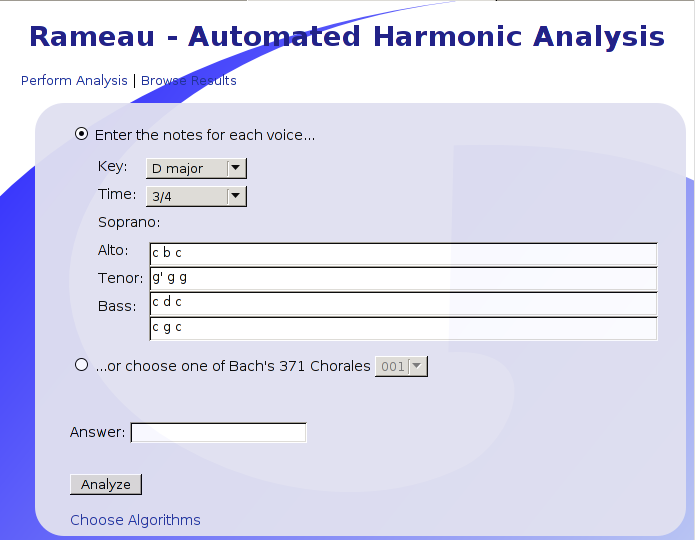
\includegraphics[scale=.5]{rameau-web}
  \caption{Rameau's web interface}
  \label{fig:rameau-web}
\end{figure*}

Rameau has nine algorithms for chord finding and four algorithms for
roman numeral analysis. Figures \ref{fig:chord-name-analysis} and
\ref{fig:roman-analysis} show the analysis result for the chord
finding and roman numeral analysis of the chorale 130 in the
Riemenschneider edition \cite{bach41:371} , respectively. Each row
shows the result for one algorithm and the last row show the expected
answer from the answer sheet. Rameau can output the result in a
text-only table or in an annotated score using LilyPond
\cite{nienhuys.ea08:LilyPond} to render the score. It is noteworthy
that the decision tree, k-nearest-neighbor, and the neural net
algorithms have a 100\% accuracy in this chorale.

The answer sheet is a simple ASCII file with the chords names or the
roman numerals. The format is familiar to students of harmony classes,
the only major difference is that the numbers to indicate intervals
are separated by a dot (where they are usually piled on top of each
other in a graphical representation). For instance, a C major chord
with 7th, 9th, and 13th is represented as C7.9.13. The following is
the complete answer sheet for the chord name analysis of chorale
\#130:

\begin{verbatim}
Em D/F# G B7/F# Em B/D# C/E D7/F# [A] Em7
Am7/C Am7 D G G G/B D D Am/C Em/B [A] B 
B7 Em
\end{verbatim}

and the complete answer sheet for the roman numeral analysis is:

\begin{verbatim}
e: i V6/III III V4.3 i V6 VI6 V6.5/III
III i G: ii6.5 ii7 V I I I6 V -
e: iv6 i6.4 - V7 - i
\end{verbatim}

\begin{figure}
  \centering
  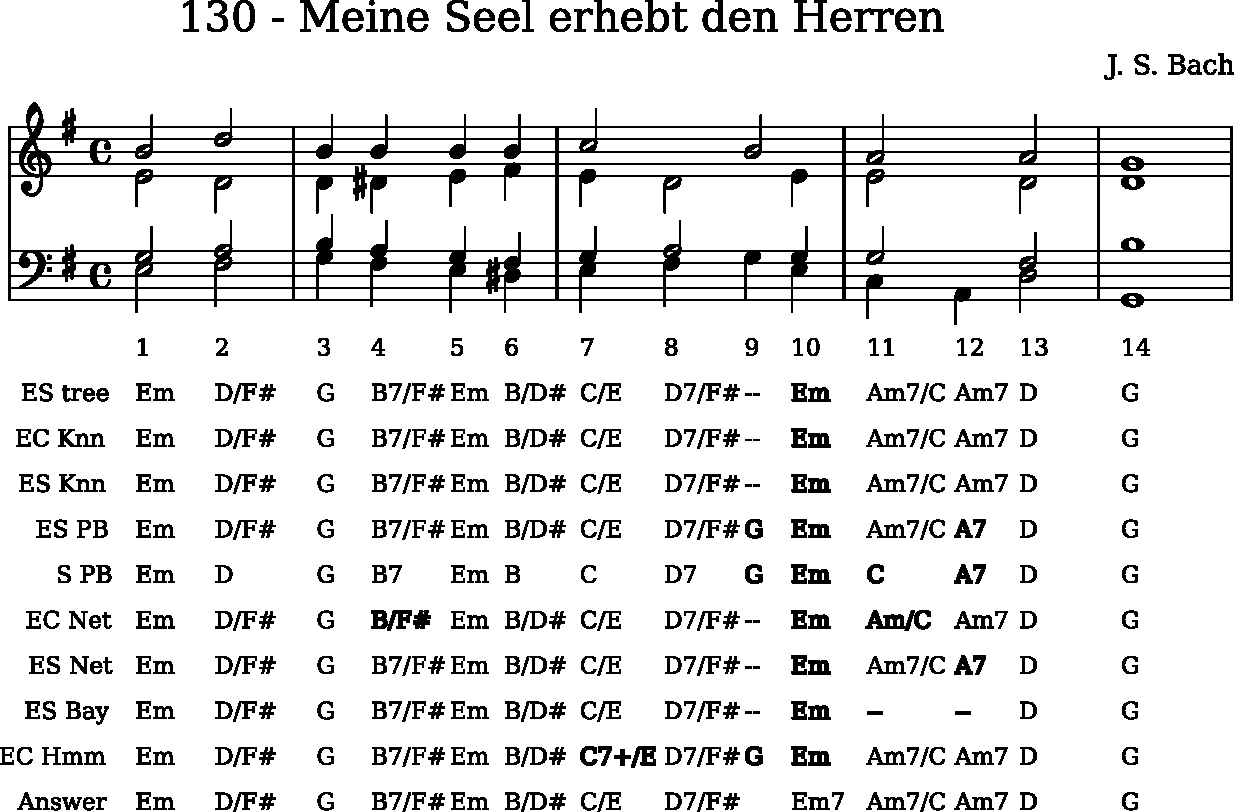
\includegraphics[scale=0.4]{analysis-130}
  \caption{Chord name analysis}
  \label{fig:chord-name-analysis}
\end{figure}
\begin{figure}
  \centering
  \includegraphics[scale=0.4]{analysis-functional-130}  
  \caption{Roman numeral analysis}
  \label{fig:roman-analysis}
\end{figure}

\section{Algorithms}
\label{sec:algorithms}

Rameau includes implementations of some chord labeling and roman
numeral analysis algorithms. Among them are a hidden Markov model
\cite{raphael.ea03:harmonic}, a reimplementation of Pardo \&
Birmingham's algorithm \cite{pardo.ea99:automated}, neural networks
\cite{tsui02:harmonic}, a port of Temperley and Sleator's ``melisma''
root-finding algorithm \cite{temperley.ea99:modeling}, and some other
machine learning techniques.

The machine learning algorithms in Rameau can be tuned by command-line
parameters, and also retrained with different data sets. Also, more
than one version of each algorithm may be compiled in Rameau, and each
such version can be specifically prepared to perform better in some
condition.

\section{Computational musicology}
\label{sec:comp-music}

%% and visualization

We have implemented a few functions for computational musicology in
Rameau. The goal is to turn Rameau into a full framework for
computational musicology in the future.

The commands ``octaves'' and ``fifths'' show how many consecutive
octaves and fifths are in a piece and where they are. These functions
can generate lilypond scores of the passage where the octaves or
fifths happens, making it easy to visualize the results. We found, for
instance, that all consecutive octaves in Bach Chorales are in the
form unison--octave or octave--unison (see fig.
\ref{fig:oitavas-e-unissonos}), but no consecutive octaves in all
Chorales are parallel, although a few fifths are (in chorales 4, 46,
71, and 266).

\begin{figure}[!h]
  \centering
  \subfloat[Chorale \#244]{
    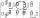
\includegraphics[scale=1]{244-oitava}
    \label{fig:244-oitava}
  }
  \qquad
  \subfloat[Chorale \#279]{
    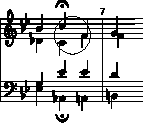
\includegraphics[scale=1]{279-oitava}
    \label{fig:279-oitava}
  }
  \qquad
  \subfloat[Chorale \#329]{
    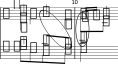
\includegraphics[scale=1]{329-oitava}
    \label{fig:329-oitava}
  }
  \caption{Consecutive octaves and unisons}
  \label{fig:oitavas-e-unissonos}
\end{figure}

The command ``chords'' list the frequency of each type of chord in a
set of chorales. For instance, we can see the type of chords in
chorale \#130 in the following list:

\begin{verbatim}
 C/F#                : 4.2% (1 of 24)
 C/D#                : 4.2% (1 of 24)
 C/E                 : 4.2% (1 of 24)
 Cm7/C               : 4.2% (1 of 24)
 Cm7                 : 4.2% (1 of 24)
 C/B                 : 4.2% (1 of 24)
 Cm/C                : 4.2% (1 of 24)
 Cm/B                : 4.2% (1 of 24)
 C7                  : 4.2% (1 of 24)
 C7/F#               : 8.3% (2 of 24)
 --                  : 8.3% (2 of 24)
 Cm                  : 16.7% (4 of 24)
 C                   : 29.2% (7 of 24)
\end{verbatim}

Not surprisingly, the major and minor triad account for the majority
of chord types. But more than 8.3\% are non-chords (marked with a
double dash), since things listed as chords like C7/F$\sharp$ and
C/D$\sharp$ are probably non-chord tones as well. With this command we
can inspect what are the most used types of sonorities, besides the
major and minor triads.

The command ``crossings'' find passages where are voice crossings. We
found that there are some kind of voice crossing in 57\% of the Bach
Chorales, although most of the crossings happen in a short period of
time (no more than two beats). There are a few interesting cases. For
instance, the alto is the lowest voice for a brief period of time in
chorale \#35 (fig. \ref{fig:035-cruzamento}) and there is a crossing
of the soprano and alto and tenor and bass at the same time in chorale
\# 290 (fig. \ref{fig:290-66-74-cruzamento}).

There are also commands to find the vocal range used in a composition,
to find melodic jumps in a voice (to analyze vocal writing, for
example), to show how the seventh of chords were resolved, and to
collect stats on how many chord progressions found in the chorales are
strong, weak, superstrong and neutral, according to Schoenberg's
theory of harmony.

\begin{figure}[!h]
  \centering
  \subfloat[Chorale \#35]{
    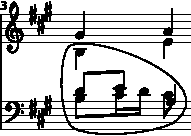
\includegraphics[scale=1]{035-16-20-cruzamento}
    \label{fig:035-cruzamento}
  }
  \subfloat[Chorale \#290]{
    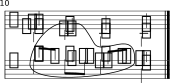
\includegraphics[scale=1]{290-66-74-cruzamento}
    \label{fig:290-66-74-cruzamento}
  }
  \caption{Voice crossing}
  \label{fig:coral-003}
\end{figure}

Finally, Rameau can analyze the final cadence of the chorales and list
then. Many commands can generate a cloud representation of its
results. The advantage of such representation is that a large amount
of data can be visualized at glance in just one picture. We can see a
cloud representation for all final cadences in the Bach Chorales in
figure \ref{fig:cadences}. From this figure it is easy to see that the
most common cadence is I ii V I, where ii can either be a minor triad
or a half-diminished seventh chord.

\begin{figure}
  \centering
  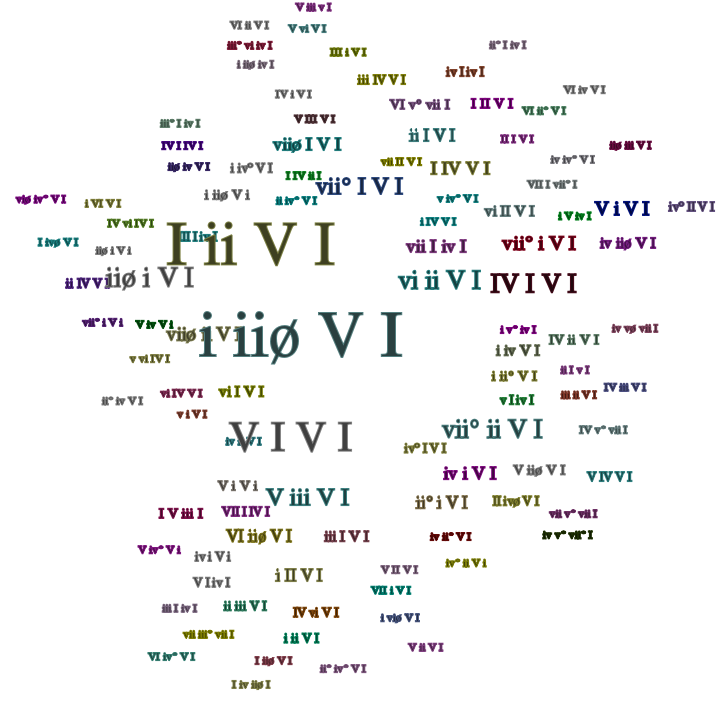
\includegraphics[scale=0.35]{cadences}
  \caption{Final cadences in Bach Chorales}
  \label{fig:cadences}
\end{figure}

\section{Conclusion and Discussion}
\label{sec:conclusion}

In this paper we presented the current status of Rameau, a framework
for automatic harmonic analysis and computational musicology. In this
framework we implemented a few algorithms for chord-labeling and roman
numeral analysis and also a few commands for computational musicology.

A system is as good as the input provided to it. Although we published
the preliminary results of using the computational musicology commands
in the 371 Bach Chorales, we found and corrected a large amount of
errors in our input data, so much that we are not comfortable in
publishing any more results until we correct the corpus to a level
that makes us more confident. We are in the process of correcting all
371 chorales against the Budapest edition, that some musicologists
find reliable \cite{fitsioris.ea08:parallel}.

Also, the functions for musicology need to be further tested, debugged,
and refined. The Rameau architecture is too tied to 4-voice part
writing. We plan to address these problems in a future release of
Rameau.

%%% Local Variables: 
%%% mode: latex
%%% TeX-master: "icmc2009"
%%% End: 


\bibliographystyle{IEEEtranS}
\bibliography{strings,harmonic-analysis,genos}

\end{document}
